\documentclass[1p]{elsarticle_modified}
%\bibliographystyle{elsarticle-num}

%\usepackage[colorlinks]{hyperref}
%\usepackage{abbrmath_seonhwa} %\Abb, \Ascr, \Acal ,\Abf, \Afrak
\usepackage{amsfonts}
\usepackage{amssymb}
\usepackage{amsmath}
\usepackage{amsthm}
\usepackage{scalefnt}
\usepackage{amsbsy}
\usepackage{kotex}
\usepackage{caption}
\usepackage{subfig}
\usepackage{color}
\usepackage{graphicx}
\usepackage{xcolor} %% white, black, red, green, blue, cyan, magenta, yellow
\usepackage{float}
\usepackage{setspace}
\usepackage{hyperref}

\usepackage{tikz}
\usetikzlibrary{arrows}

\usepackage{multirow}
\usepackage{array} % fixed length table
\usepackage{hhline}

%%%%%%%%%%%%%%%%%%%%%
\makeatletter
\renewcommand*\env@matrix[1][\arraystretch]{%
	\edef\arraystretch{#1}%
	\hskip -\arraycolsep
	\let\@ifnextchar\new@ifnextchar
	\array{*\c@MaxMatrixCols c}}
\makeatother %https://tex.stackexchange.com/questions/14071/how-can-i-increase-the-line-spacing-in-a-matrix
%%%%%%%%%%%%%%%

\usepackage[normalem]{ulem}

\newcommand{\msout}[1]{\ifmmode\text{\sout{\ensuremath{#1}}}\else\sout{#1}\fi}
%SOURCE: \msout is \stkout macro in https://tex.stackexchange.com/questions/20609/strikeout-in-math-mode

\newcommand{\cancel}[1]{
	\ifmmode
	{\color{red}\msout{#1}}
	\else
	{\color{red}\sout{#1}}
	\fi
}

\newcommand{\add}[1]{
	{\color{blue}\uwave{#1}}
}

\newcommand{\replace}[2]{
	\ifmmode
	{\color{red}\msout{#1}}{\color{blue}\uwave{#2}}
	\else
	{\color{red}\sout{#1}}{\color{blue}\uwave{#2}}
	\fi
}

\newcommand{\Sol}{\mathcal{S}} %segment
\newcommand{\D}{D} %diagram
\newcommand{\A}{\mathcal{A}} %arc


%%%%%%%%%%%%%%%%%%%%%%%%%%%%%5 test

\def\sl{\operatorname{\textup{SL}}(2,\Cbb)}
\def\psl{\operatorname{\textup{PSL}}(2,\Cbb)}
\def\quan{\mkern 1mu \triangleright \mkern 1mu}

\theoremstyle{definition}
\newtheorem{thm}{Theorem}[section]
\newtheorem{prop}[thm]{Proposition}
\newtheorem{lem}[thm]{Lemma}
\newtheorem{ques}[thm]{Question}
\newtheorem{cor}[thm]{Corollary}
\newtheorem{defn}[thm]{Definition}
\newtheorem{exam}[thm]{Example}
\newtheorem{rmk}[thm]{Remark}
\newtheorem{alg}[thm]{Algorithm}

\newcommand{\I}{\sqrt{-1}}
\begin{document}

%\begin{frontmatter}
%
%\title{Boundary parabolic representations of knots up to 8 crossings}
%
%%% Group authors per affiliation:
%\author{Yunhi Cho} 
%\address{Department of Mathematics, University of Seoul, Seoul, Korea}
%\ead{yhcho@uos.ac.kr}
%
%
%\author{Seonhwa Kim} %\fnref{s_kim}}
%\address{Center for Geometry and Physics, Institute for Basic Science, Pohang, 37673, Korea}
%\ead{ryeona17@ibs.re.kr}
%
%\author{Hyuk Kim}
%\address{Department of Mathematical Sciences, Seoul National University, Seoul 08826, Korea}
%\ead{hyukkim@snu.ac.kr}
%
%\author{Seokbeom Yoon}
%\address{Department of Mathematical Sciences, Seoul National University, Seoul, 08826,  Korea}
%\ead{sbyoon15@snu.ac.kr}
%
%\begin{abstract}
%We find all boundary parabolic representation of knots up to 8 crossings.
%
%\end{abstract}
%\begin{keyword}
%    \MSC[2010] 57M25 
%\end{keyword}
%
%\end{frontmatter}

%\linenumbers
%\tableofcontents
%
\newcommand\colored[1]{\textcolor{white}{\rule[-0.35ex]{0.8em}{1.4ex}}\kern-0.8em\color{red} #1}%
%\newcommand\colored[1]{\textcolor{white}{ #1}\kern-2.17ex	\textcolor{white}{ #1}\kern-1.81ex	\textcolor{white}{ #1}\kern-2.15ex\color{red}#1	}

{\Large $\underline{12n_{0071}~(K12n_{0071})}$}

\setlength{\tabcolsep}{10pt}
\renewcommand{\arraystretch}{1.6}
\vspace{1cm}\begin{tabular}{m{100pt}>{\centering\arraybackslash}m{274pt}}
\multirow{5}{120pt}{
	\centering
	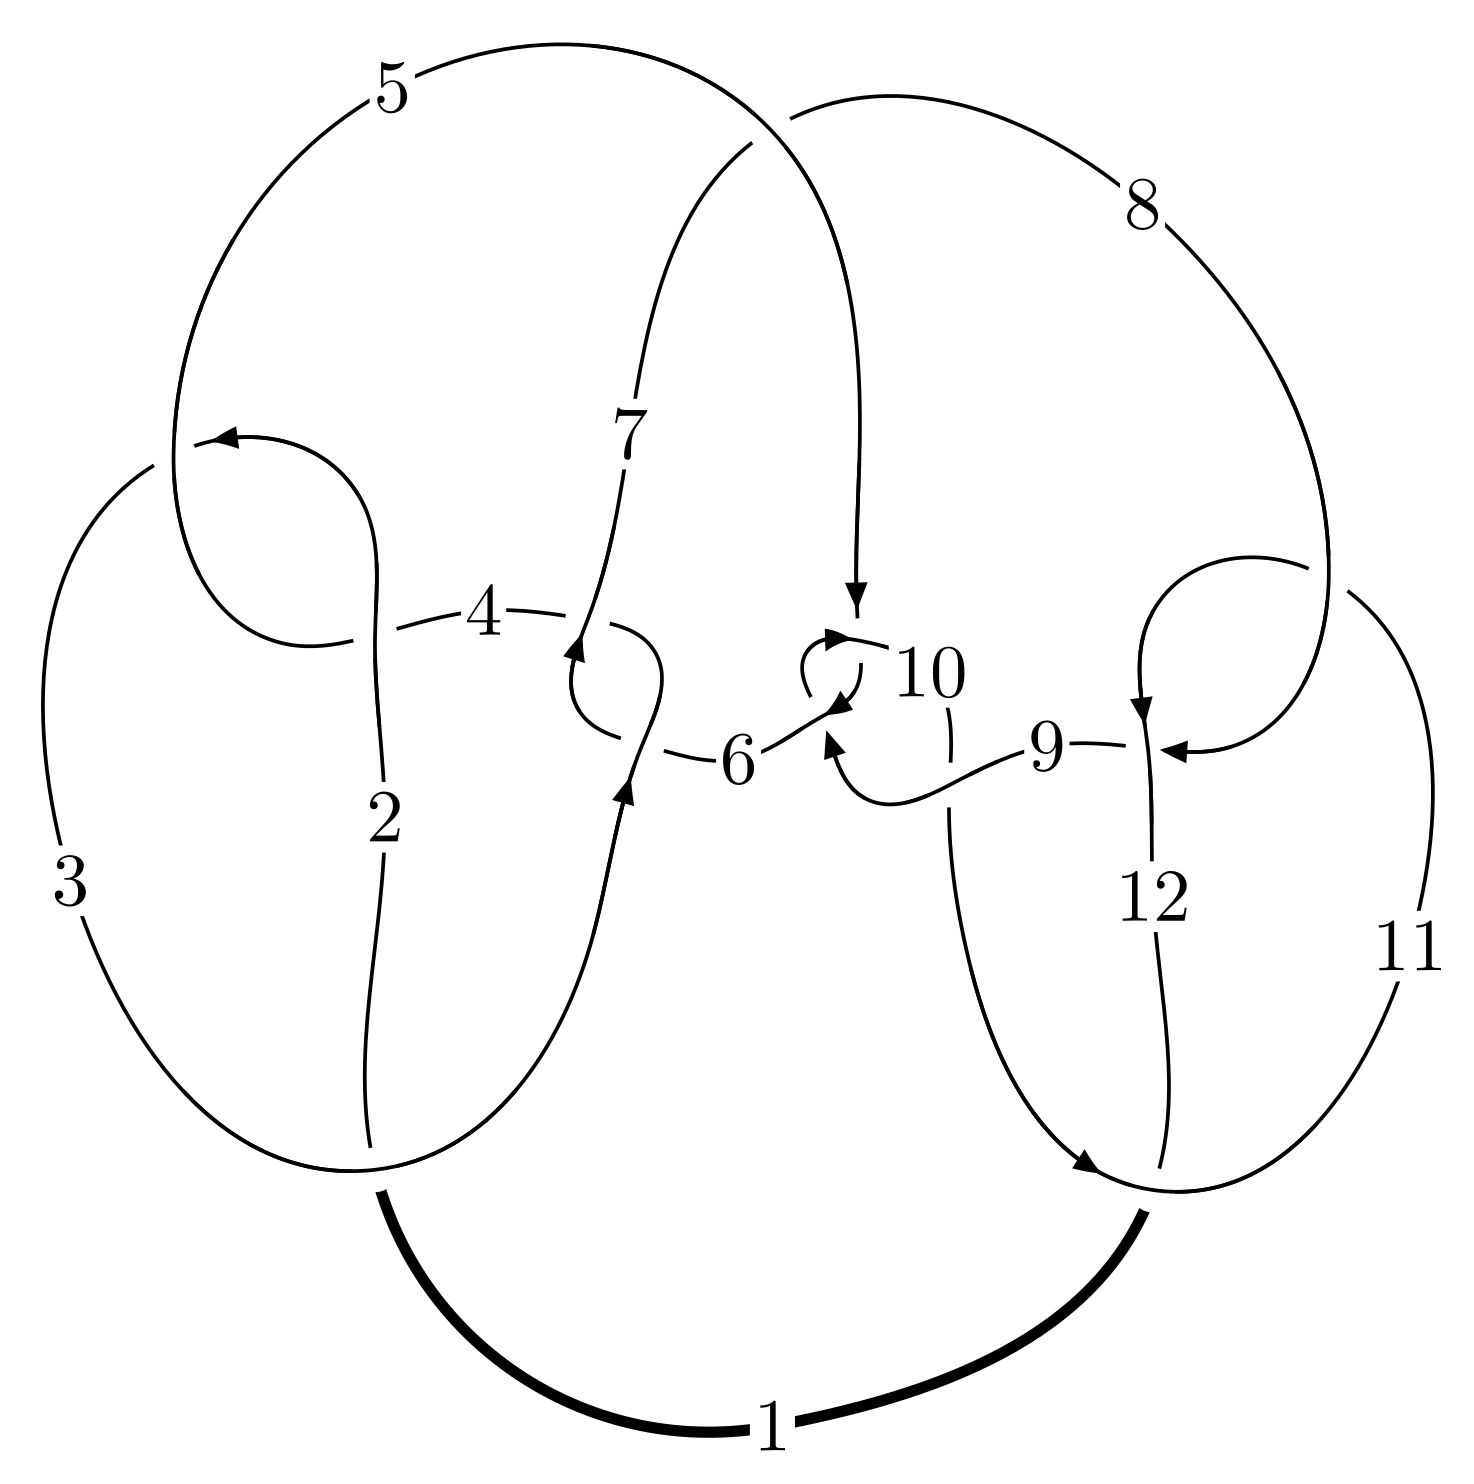
\includegraphics[width=112pt]{../../../GIT/diagram.site/Diagrams/png/2160_12n_0071.png}\\
\ \ \ A knot diagram\footnotemark}&
\allowdisplaybreaks
\textbf{Linearized knot diagam} \\
\cline{2-2}
 &
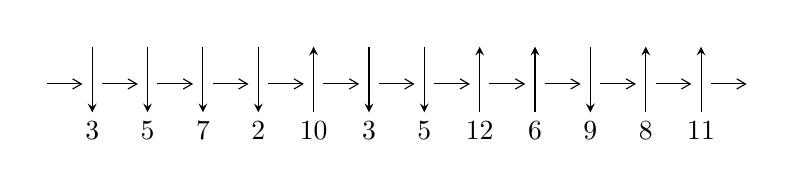
\begin{tikzpicture}[x=20pt, y=17pt]
	% nodes
	\node (C0) at (0, 0) {};
	\node (C1) at (1, 0) {};
	\node (C1U) at (1, +1) {};
	\node (C1D) at (1, -1) {3};

	\node (C2) at (2, 0) {};
	\node (C2U) at (2, +1) {};
	\node (C2D) at (2, -1) {5};

	\node (C3) at (3, 0) {};
	\node (C3U) at (3, +1) {};
	\node (C3D) at (3, -1) {7};

	\node (C4) at (4, 0) {};
	\node (C4U) at (4, +1) {};
	\node (C4D) at (4, -1) {2};

	\node (C5) at (5, 0) {};
	\node (C5U) at (5, +1) {};
	\node (C5D) at (5, -1) {10};

	\node (C6) at (6, 0) {};
	\node (C6U) at (6, +1) {};
	\node (C6D) at (6, -1) {3};

	\node (C7) at (7, 0) {};
	\node (C7U) at (7, +1) {};
	\node (C7D) at (7, -1) {5};

	\node (C8) at (8, 0) {};
	\node (C8U) at (8, +1) {};
	\node (C8D) at (8, -1) {12};

	\node (C9) at (9, 0) {};
	\node (C9U) at (9, +1) {};
	\node (C9D) at (9, -1) {6};

	\node (C10) at (10, 0) {};
	\node (C10U) at (10, +1) {};
	\node (C10D) at (10, -1) {9};

	\node (C11) at (11, 0) {};
	\node (C11U) at (11, +1) {};
	\node (C11D) at (11, -1) {8};

	\node (C12) at (12, 0) {};
	\node (C12U) at (12, +1) {};
	\node (C12D) at (12, -1) {11};
	\node (C13) at (13, 0) {};

	% arrows
	\draw[->,>={angle 60}]
	(C0) edge (C1) (C1) edge (C2) (C2) edge (C3) (C3) edge (C4) (C4) edge (C5) (C5) edge (C6) (C6) edge (C7) (C7) edge (C8) (C8) edge (C9) (C9) edge (C10) (C10) edge (C11) (C11) edge (C12) (C12) edge (C13) ;	\draw[->,>=stealth]
	(C1U) edge (C1D) (C2U) edge (C2D) (C3U) edge (C3D) (C4U) edge (C4D) (C5D) edge (C5U) (C6U) edge (C6D) (C7U) edge (C7D) (C8D) edge (C8U) (C9D) edge (C9U) (C10U) edge (C10D) (C11D) edge (C11U) (C12D) edge (C12U) ;
	\end{tikzpicture} \\
\hhline{~~} \\& 
\textbf{Solving Sequence} \\ \cline{2-2} 
 &
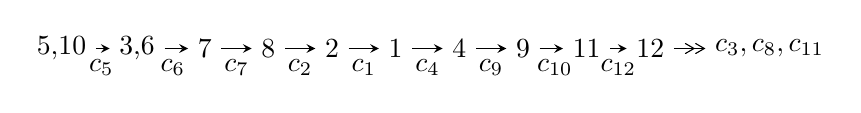
\begin{tikzpicture}[x=23pt, y=7pt]
	% node
	\node (A0) at (-1/8, 0) {5,10};
	\node (A1) at (17/16, 0) {3,6};
	\node (A2) at (17/8, 0) {7};
	\node (A3) at (25/8, 0) {8};
	\node (A4) at (33/8, 0) {2};
	\node (A5) at (41/8, 0) {1};
	\node (A6) at (49/8, 0) {4};
	\node (A7) at (57/8, 0) {9};
	\node (A8) at (65/8, 0) {11};
	\node (A9) at (73/8, 0) {12};
	\node (C1) at (1/2, -1) {$c_{5}$};
	\node (C2) at (13/8, -1) {$c_{6}$};
	\node (C3) at (21/8, -1) {$c_{7}$};
	\node (C4) at (29/8, -1) {$c_{2}$};
	\node (C5) at (37/8, -1) {$c_{1}$};
	\node (C6) at (45/8, -1) {$c_{4}$};
	\node (C7) at (53/8, -1) {$c_{9}$};
	\node (C8) at (61/8, -1) {$c_{10}$};
	\node (C9) at (69/8, -1) {$c_{12}$};
	\node (A10) at (11, 0) {$c_{3},c_{8},c_{11}$};

	% edge
	\draw[->,>=stealth]	
	(A0) edge (A1) (A1) edge (A2) (A2) edge (A3) (A3) edge (A4) (A4) edge (A5) (A5) edge (A6) (A6) edge (A7) (A7) edge (A8) (A8) edge (A9) ;
	\draw[->>,>={angle 60}]	
	(A9) edge (A10);
\end{tikzpicture} \\ 

\end{tabular} \\

\footnotetext{
The image of knot diagram is generated by the software ``\textbf{Draw programme}" developed by Andrew Bartholomew(\url{http://www.layer8.co.uk/maths/draw/index.htm\#Running-draw}), where we modified some parts for our purpose(\url{https://github.com/CATsTAILs/LinksPainter}).
}\phantom \\ \newline 
\centering \textbf{Ideals for irreducible components\footnotemark of $X_{\text{par}}$} 
 
\begin{align*}
I^u_{1}&=\langle 
-1.70615\times10^{34} u^{39}+1.06745\times10^{33} u^{38}+\cdots+5.47651\times10^{34} b+1.26128\times10^{35},\\
\phantom{I^u_{1}}&\phantom{= \langle  }-1.54680\times10^{35} u^{39}+2.39864\times10^{35} u^{38}+\cdots+1.09530\times10^{35} a-4.53620\times10^{35},\;u^{40}-2 u^{39}+\cdots+4 u-4\rangle \\
I^u_{2}&=\langle 
b+1,\;- u^8+2 u^7-3 u^6+3 u^5-4 u^4+4 u^3-3 u^2+a+2 u-1,\;u^9- u^8+2 u^7- u^6+3 u^5- u^4+2 u^3+u+1\rangle \\
\\
I^v_{1}&=\langle 
a,\;b+v-2,\;v^2-3 v+1\rangle \\
\end{align*}
\raggedright * 3 irreducible components of $\dim_{\mathbb{C}}=0$, with total 51 representations.\\
\footnotetext{All coefficients of polynomials are rational numbers. But the coefficients are sometimes approximated in decimal forms when there is not enough margin.}
\newpage
\renewcommand{\arraystretch}{1}
\centering \section*{I. $I^u_{1}= \langle -1.71\times10^{34} u^{39}+1.07\times10^{33} u^{38}+\cdots+5.48\times10^{34} b+1.26\times10^{35},\;-1.55\times10^{35} u^{39}+2.40\times10^{35} u^{38}+\cdots+1.10\times10^{35} a-4.54\times10^{35},\;u^{40}-2 u^{39}+\cdots+4 u-4 \rangle$}
\flushleft \textbf{(i) Arc colorings}\\
\begin{tabular}{m{7pt} m{180pt} m{7pt} m{180pt} }
\flushright $a_{5}=$&$\begin{pmatrix}1\\0\end{pmatrix}$ \\
\flushright $a_{10}=$&$\begin{pmatrix}0\\u\end{pmatrix}$ \\
\flushright $a_{3}=$&$\begin{pmatrix}1.41222 u^{39}-2.18994 u^{38}+\cdots-11.0073 u+4.14151\\0.311540 u^{39}-0.0194914 u^{38}+\cdots-2.46184 u-2.30307\end{pmatrix}$ \\
\flushright $a_{6}=$&$\begin{pmatrix}1\\- u^2\end{pmatrix}$ \\
\flushright $a_{7}=$&$\begin{pmatrix}1.29467 u^{39}-2.32830 u^{38}+\cdots-7.27281 u+5.25464\\0.739952 u^{39}-0.868974 u^{38}+\cdots-6.01405 u-0.199281\end{pmatrix}$ \\
\flushright $a_{8}=$&$\begin{pmatrix}0.554717 u^{39}-1.45933 u^{38}+\cdots-1.25876 u+5.45392\\0.739952 u^{39}-0.868974 u^{38}+\cdots-6.01405 u-0.199281\end{pmatrix}$ \\
\flushright $a_{2}=$&$\begin{pmatrix}1.72376 u^{39}-2.20943 u^{38}+\cdots-13.4692 u+1.83844\\0.311540 u^{39}-0.0194914 u^{38}+\cdots-2.46184 u-2.30307\end{pmatrix}$ \\
\flushright $a_{1}=$&$\begin{pmatrix}1.29467 u^{39}-2.32830 u^{38}+\cdots-7.27281 u+5.25464\\-0.230688 u^{39}+0.321263 u^{38}+\cdots+1.87952 u-0.844865\end{pmatrix}$ \\
\flushright $a_{4}=$&$\begin{pmatrix}0.544195 u^{39}-0.801448 u^{38}+\cdots-5.22381 u+0.269369\\-0.448480 u^{39}+0.683873 u^{38}+\cdots+4.04346 u-1.80083\end{pmatrix}$ \\
\flushright $a_{9}=$&$\begin{pmatrix}- u\\u^3+u\end{pmatrix}$ \\
\flushright $a_{11}=$&$\begin{pmatrix}- u^3\\u^5+u^3+u\end{pmatrix}$ \\
\flushright $a_{12}=$&$\begin{pmatrix}1.23672 u^{39}-2.44708 u^{38}+\cdots-6.97510 u+6.29059\\-0.392051 u^{39}+0.485888 u^{38}+\cdots+3.56359 u-0.624191\end{pmatrix}$\\&\end{tabular}
\flushleft \textbf{(ii) Obstruction class $= -1$}\\~\\
\flushleft \textbf{(iii) Cusp Shapes $= 0.979451 u^{39}-1.42354 u^{38}+\cdots+1.47042 u-2.27161$}\\~\\
\newpage\renewcommand{\arraystretch}{1}
\flushleft \textbf{(iv) u-Polynomials at the component}\newline \\
\begin{tabular}{m{50pt}|m{274pt}}
Crossings & \hspace{64pt}u-Polynomials at each crossing \\
\hline $$\begin{aligned}c_{1}\end{aligned}$$&$\begin{aligned}
&u^{40}+57 u^{39}+\cdots+351 u+1
\end{aligned}$\\
\hline $$\begin{aligned}c_{2},c_{4}\end{aligned}$$&$\begin{aligned}
&u^{40}-11 u^{39}+\cdots+9 u+1
\end{aligned}$\\
\hline $$\begin{aligned}c_{3},c_{6}\end{aligned}$$&$\begin{aligned}
&u^{40}+2 u^{39}+\cdots+512 u-512
\end{aligned}$\\
\hline $$\begin{aligned}c_{5},c_{9}\end{aligned}$$&$\begin{aligned}
&u^{40}-2 u^{39}+\cdots+4 u-4
\end{aligned}$\\
\hline $$\begin{aligned}c_{7}\end{aligned}$$&$\begin{aligned}
&u^{40}-3 u^{39}+\cdots+u-1
\end{aligned}$\\
\hline $$\begin{aligned}c_{8},c_{11}\end{aligned}$$&$\begin{aligned}
&u^{40}+4 u^{39}+\cdots-6 u+1
\end{aligned}$\\
\hline $$\begin{aligned}c_{10}\end{aligned}$$&$\begin{aligned}
&u^{40}+18 u^{39}+\cdots-104 u+16
\end{aligned}$\\
\hline $$\begin{aligned}c_{12}\end{aligned}$$&$\begin{aligned}
&u^{40}-20 u^{39}+\cdots-94 u+1
\end{aligned}$\\
\hline
\end{tabular}\\~\\
\newpage\renewcommand{\arraystretch}{1}
\flushleft \textbf{(v) Riley Polynomials at the component}\newline \\
\begin{tabular}{m{50pt}|m{274pt}}
Crossings & \hspace{64pt}Riley Polynomials at each crossing \\
\hline $$\begin{aligned}c_{1}\end{aligned}$$&$\begin{aligned}
&y^{40}-137 y^{39}+\cdots-102695 y+1
\end{aligned}$\\
\hline $$\begin{aligned}c_{2},c_{4}\end{aligned}$$&$\begin{aligned}
&y^{40}-57 y^{39}+\cdots-351 y+1
\end{aligned}$\\
\hline $$\begin{aligned}c_{3},c_{6}\end{aligned}$$&$\begin{aligned}
&y^{40}-60 y^{39}+\cdots-3407872 y+262144
\end{aligned}$\\
\hline $$\begin{aligned}c_{5},c_{9}\end{aligned}$$&$\begin{aligned}
&y^{40}+18 y^{39}+\cdots-104 y+16
\end{aligned}$\\
\hline $$\begin{aligned}c_{7}\end{aligned}$$&$\begin{aligned}
&y^{40}-85 y^{39}+\cdots-31 y+1
\end{aligned}$\\
\hline $$\begin{aligned}c_{8},c_{11}\end{aligned}$$&$\begin{aligned}
&y^{40}-20 y^{39}+\cdots-94 y+1
\end{aligned}$\\
\hline $$\begin{aligned}c_{10}\end{aligned}$$&$\begin{aligned}
&y^{40}+6 y^{39}+\cdots-26912 y+256
\end{aligned}$\\
\hline $$\begin{aligned}c_{12}\end{aligned}$$&$\begin{aligned}
&y^{40}+4 y^{39}+\cdots-7630 y+1
\end{aligned}$\\
\hline
\end{tabular}\\~\\
\newpage\flushleft \textbf{(vi) Complex Volumes and Cusp Shapes}
$$\begin{array}{c|c|c}  
\text{Solutions to }I^u_{1}& \I (\text{vol} + \sqrt{-1}CS) & \text{Cusp shape}\\
 \hline 
\begin{aligned}
u &= -0.767555 + 0.682797 I \\
a &= \phantom{-}0.527466 - 0.374649 I \\
b &= \phantom{-}0.351491 + 0.041737 I\end{aligned}
 & \phantom{-}3.81537 + 1.27262 I & \phantom{-}6.29824 - 0.66128 I \\ \hline\begin{aligned}
u &= -0.767555 - 0.682797 I \\
a &= \phantom{-}0.527466 + 0.374649 I \\
b &= \phantom{-}0.351491 - 0.041737 I\end{aligned}
 & \phantom{-}3.81537 - 1.27262 I & \phantom{-}6.29824 + 0.66128 I \\ \hline\begin{aligned}
u &= \phantom{-}0.873000 + 0.401971 I \\
a &= \phantom{-}0.540073 + 0.763124 I \\
b &= -0.870382 - 0.585645 I\end{aligned}
 & \phantom{-}0.09726 - 2.75203 I & -2.88480 + 4.23304 I \\ \hline\begin{aligned}
u &= \phantom{-}0.873000 - 0.401971 I \\
a &= \phantom{-}0.540073 - 0.763124 I \\
b &= -0.870382 + 0.585645 I\end{aligned}
 & \phantom{-}0.09726 + 2.75203 I & -2.88480 - 4.23304 I \\ \hline\begin{aligned}
u &= \phantom{-}0.552365 + 0.888486 I \\
a &= \phantom{-}0.518410 + 0.192533 I \\
b &= \phantom{-}0.342558 + 0.168348 I\end{aligned}
 & \phantom{-}0.08572 + 2.19817 I & \phantom{-}0.38918 - 2.62021 I \\ \hline\begin{aligned}
u &= \phantom{-}0.552365 - 0.888486 I \\
a &= \phantom{-}0.518410 - 0.192533 I \\
b &= \phantom{-}0.342558 - 0.168348 I\end{aligned}
 & \phantom{-}0.08572 - 2.19817 I & \phantom{-}0.38918 + 2.62021 I \\ \hline\begin{aligned}
u &= -0.027732 + 0.938035 I \\
a &= \phantom{-}0.600853 - 0.094307 I \\
b &= -0.017454 + 0.471847 I\end{aligned}
 & -1.55152 + 1.36538 I & -4.32744 - 4.03663 I \\ \hline\begin{aligned}
u &= -0.027732 - 0.938035 I \\
a &= \phantom{-}0.600853 + 0.094307 I \\
b &= -0.017454 - 0.471847 I\end{aligned}
 & -1.55152 - 1.36538 I & -4.32744 + 4.03663 I \\ \hline\begin{aligned}
u &= \phantom{-}0.431539 + 0.988175 I \\
a &= \phantom{-}0.546146 + 0.283746 I \\
b &= -0.284057 - 0.713228 I\end{aligned}
 & -0.42853 + 2.82368 I & -2.74140 - 3.00000 I \\ \hline\begin{aligned}
u &= \phantom{-}0.431539 - 0.988175 I \\
a &= \phantom{-}0.546146 - 0.283746 I \\
b &= -0.284057 + 0.713228 I\end{aligned}
 & -0.42853 - 2.82368 I & -2.74140 + 3.00000 I\\
 \hline 
 \end{array}$$\newpage$$\begin{array}{c|c|c}  
\text{Solutions to }I^u_{1}& \I (\text{vol} + \sqrt{-1}CS) & \text{Cusp shape}\\
 \hline 
\begin{aligned}
u &= -1.079360 + 0.315602 I \\
a &= \phantom{-}0.188664 + 0.002235 I \\
b &= \phantom{-}1.79704 - 0.10786 I\end{aligned}
 & -11.27530 + 1.20929 I & -5.80586 + 0.92387 I \\ \hline\begin{aligned}
u &= -1.079360 - 0.315602 I \\
a &= \phantom{-}0.188664 - 0.002235 I \\
b &= \phantom{-}1.79704 + 0.10786 I\end{aligned}
 & -11.27530 - 1.20929 I & -5.80586 - 0.92387 I \\ \hline\begin{aligned}
u &= \phantom{-}0.216652 + 1.135450 I \\
a &= -1.66179 - 0.18633 I \\
b &= -1.318890 - 0.413598 I\end{aligned}
 & -5.01603 - 0.16820 I & -8.63543 + 0.05327 I \\ \hline\begin{aligned}
u &= \phantom{-}0.216652 - 1.135450 I \\
a &= -1.66179 + 0.18633 I \\
b &= -1.318890 + 0.413598 I\end{aligned}
 & -5.01603 + 0.16820 I & -8.63543 - 0.05327 I \\ \hline\begin{aligned}
u &= \phantom{-}0.481478 + 1.060550 I \\
a &= \phantom{-}2.09296 + 1.81237 I \\
b &= \phantom{-}1.77358 - 0.16425 I\end{aligned}
 & -8.56336 + 3.34791 I & -4.12753 - 2.29966 I \\ \hline\begin{aligned}
u &= \phantom{-}0.481478 - 1.060550 I \\
a &= \phantom{-}2.09296 - 1.81237 I \\
b &= \phantom{-}1.77358 + 0.16425 I\end{aligned}
 & -8.56336 - 3.34791 I & -4.12753 + 2.29966 I \\ \hline\begin{aligned}
u &= -0.389413 + 1.130570 I \\
a &= -1.39760 + 0.84641 I \\
b &= -1.016230 - 0.711563 I\end{aligned}
 & -4.30445 - 2.98930 I & -8.10205 + 2.51738 I \\ \hline\begin{aligned}
u &= -0.389413 - 1.130570 I \\
a &= -1.39760 - 0.84641 I \\
b &= -1.016230 + 0.711563 I\end{aligned}
 & -4.30445 + 2.98930 I & -8.10205 - 2.51738 I \\ \hline\begin{aligned}
u &= -0.697362 + 1.004410 I \\
a &= \phantom{-}0.423595 - 0.213085 I \\
b &= \phantom{-}0.479221 - 0.154409 I\end{aligned}
 & \phantom{-}2.84493 - 6.83482 I & \phantom{-}4.23533 + 5.20206 I \\ \hline\begin{aligned}
u &= -0.697362 - 1.004410 I \\
a &= \phantom{-}0.423595 + 0.213085 I \\
b &= \phantom{-}0.479221 + 0.154409 I\end{aligned}
 & \phantom{-}2.84493 + 6.83482 I & \phantom{-}4.23533 - 5.20206 I\\
 \hline 
 \end{array}$$\newpage$$\begin{array}{c|c|c}  
\text{Solutions to }I^u_{1}& \I (\text{vol} + \sqrt{-1}CS) & \text{Cusp shape}\\
 \hline 
\begin{aligned}
u &= -0.496749 + 1.146130 I \\
a &= -1.36151 + 0.53213 I \\
b &= -1.45579 + 0.29115 I\end{aligned}
 & -3.51298 - 4.94394 I & -5.28672 + 5.25390 I \\ \hline\begin{aligned}
u &= -0.496749 - 1.146130 I \\
a &= -1.36151 - 0.53213 I \\
b &= -1.45579 - 0.29115 I\end{aligned}
 & -3.51298 + 4.94394 I & -5.28672 - 5.25390 I \\ \hline\begin{aligned}
u &= \phantom{-}1.125440 + 0.571611 I \\
a &= \phantom{-}0.189635 - 0.004384 I \\
b &= \phantom{-}1.78560 + 0.20613 I\end{aligned}
 & -9.38333 - 6.25287 I & -3.71429 + 3.55273 I \\ \hline\begin{aligned}
u &= \phantom{-}1.125440 - 0.571611 I \\
a &= \phantom{-}0.189635 + 0.004384 I \\
b &= \phantom{-}1.78560 - 0.20613 I\end{aligned}
 & -9.38333 + 6.25287 I & -3.71429 - 3.55273 I \\ \hline\begin{aligned}
u &= -0.711358 + 0.187576 I \\
a &= \phantom{-}0.28261 + 1.89131 I \\
b &= -1.119340 - 0.213535 I\end{aligned}
 & -0.733261 + 0.420305 I & -2.53134 - 5.06503 I \\ \hline\begin{aligned}
u &= -0.711358 - 0.187576 I \\
a &= \phantom{-}0.28261 - 1.89131 I \\
b &= -1.119340 + 0.213535 I\end{aligned}
 & -0.733261 - 0.420305 I & -2.53134 + 5.06503 I \\ \hline\begin{aligned}
u &= \phantom{-}0.452397 + 0.566444 I \\
a &= \phantom{-}0.191549 - 0.000487 I \\
b &= \phantom{-}1.59905 + 0.08829 I\end{aligned}
 & -6.90633 + 0.62272 I & -3.96477 - 7.65597 I \\ \hline\begin{aligned}
u &= \phantom{-}0.452397 - 0.566444 I \\
a &= \phantom{-}0.191549 + 0.000487 I \\
b &= \phantom{-}1.59905 - 0.08829 I\end{aligned}
 & -6.90633 - 0.62272 I & -3.96477 + 7.65597 I \\ \hline\begin{aligned}
u &= \phantom{-}0.344447 + 0.623097 I \\
a &= -2.15466 - 2.41727 I \\
b &= -0.764103 + 0.413686 I\end{aligned}
 & \phantom{-}0.797208 + 0.661473 I & -4.69435 - 5.79725 I \\ \hline\begin{aligned}
u &= \phantom{-}0.344447 - 0.623097 I \\
a &= -2.15466 + 2.41727 I \\
b &= -0.764103 - 0.413686 I\end{aligned}
 & \phantom{-}0.797208 - 0.661473 I & -4.69435 + 5.79725 I\\
 \hline 
 \end{array}$$\newpage$$\begin{array}{c|c|c}  
\text{Solutions to }I^u_{1}& \I (\text{vol} + \sqrt{-1}CS) & \text{Cusp shape}\\
 \hline 
\begin{aligned}
u &= \phantom{-}0.608559 + 1.157670 I \\
a &= -1.08482 - 0.95472 I \\
b &= -0.923559 + 0.844828 I\end{aligned}
 & -2.24385 + 8.24833 I & -4.49922 - 6.95806 I \\ \hline\begin{aligned}
u &= \phantom{-}0.608559 - 1.157670 I \\
a &= -1.08482 + 0.95472 I \\
b &= -0.923559 - 0.844828 I\end{aligned}
 & -2.24385 - 8.24833 I & -4.49922 + 6.95806 I \\ \hline\begin{aligned}
u &= -0.640898 + 1.241650 I \\
a &= \phantom{-}1.47950 - 1.37909 I \\
b &= \phantom{-}1.82246 + 0.25034 I\end{aligned}
 & -14.2021 - 7.3246 I & -7.52732 + 3.21849 I \\ \hline\begin{aligned}
u &= -0.640898 - 1.241650 I \\
a &= \phantom{-}1.47950 + 1.37909 I \\
b &= \phantom{-}1.82246 - 0.25034 I\end{aligned}
 & -14.2021 + 7.3246 I & -7.52732 - 3.21849 I \\ \hline\begin{aligned}
u &= -0.11613 + 1.42102 I \\
a &= \phantom{-}2.07367 - 0.26407 I \\
b &= \phantom{-}1.93738 + 0.04804 I\end{aligned}
 & -17.7940 - 3.0498 I & -8.36562 + 2.61097 I \\ \hline\begin{aligned}
u &= -0.11613 - 1.42102 I \\
a &= \phantom{-}2.07367 + 0.26407 I \\
b &= \phantom{-}1.93738 - 0.04804 I\end{aligned}
 & -17.7940 + 3.0498 I & -8.36562 - 2.61097 I \\ \hline\begin{aligned}
u &= \phantom{-}0.77397 + 1.20805 I \\
a &= \phantom{-}1.18273 + 1.46175 I \\
b &= \phantom{-}1.78706 - 0.30179 I\end{aligned}
 & -11.4479 + 13.0879 I & \phantom{-0.000000 } 0. - 6.81590 I \\ \hline\begin{aligned}
u &= \phantom{-}0.77397 - 1.20805 I \\
a &= \phantom{-}1.18273 - 1.46175 I \\
b &= \phantom{-}1.78706 + 0.30179 I\end{aligned}
 & -11.4479 - 13.0879 I & \phantom{-0.000000 -}0. + 6.81590 I \\ \hline\begin{aligned}
u &= \phantom{-}0.458630\phantom{ +0.000000I} \\
a &= \phantom{-}1.38775\phantom{ +0.000000I} \\
b &= -0.0558807\phantom{ +0.000000I}\end{aligned}
 & \phantom{-}1.26099\phantom{ +0.000000I} & \phantom{-}8.96990\phantom{ +0.000000I} \\ \hline\begin{aligned}
u &= -0.325204\phantom{ +0.000000I} \\
a &= \phantom{-}1.75723\phantom{ +0.000000I} \\
b &= -0.755372\phantom{ +0.000000I}\end{aligned}
 & -1.11358\phantom{ +0.000000I} & -9.07280\phantom{ +0.000000I}\\
 \hline 
 \end{array}$$\newpage\newpage\renewcommand{\arraystretch}{1}
\centering \section*{II. $I^u_{2}= \langle b+1,\;- u^8+2 u^7+\cdots+a-1,\;u^9- u^8+2 u^7- u^6+3 u^5- u^4+2 u^3+u+1 \rangle$}
\flushleft \textbf{(i) Arc colorings}\\
\begin{tabular}{m{7pt} m{180pt} m{7pt} m{180pt} }
\flushright $a_{5}=$&$\begin{pmatrix}1\\0\end{pmatrix}$ \\
\flushright $a_{10}=$&$\begin{pmatrix}0\\u\end{pmatrix}$ \\
\flushright $a_{3}=$&$\begin{pmatrix}u^8-2 u^7+3 u^6-3 u^5+4 u^4-4 u^3+3 u^2-2 u+1\\-1\end{pmatrix}$ \\
\flushright $a_{6}=$&$\begin{pmatrix}1\\- u^2\end{pmatrix}$ \\
\flushright $a_{7}=$&$\begin{pmatrix}1\\- u^2\end{pmatrix}$ \\
\flushright $a_{8}=$&$\begin{pmatrix}u^2+1\\- u^2\end{pmatrix}$ \\
\flushright $a_{2}=$&$\begin{pmatrix}u^8-2 u^7+3 u^6-3 u^5+4 u^4-4 u^3+3 u^2-2 u\\-1\end{pmatrix}$ \\
\flushright $a_{1}=$&$\begin{pmatrix}-1\\0\end{pmatrix}$ \\
\flushright $a_{4}=$&$\begin{pmatrix}u^8-2 u^7+3 u^6-3 u^5+4 u^4-4 u^3+3 u^2-2 u+1\\-1\end{pmatrix}$ \\
\flushright $a_{9}=$&$\begin{pmatrix}- u\\u^3+u\end{pmatrix}$ \\
\flushright $a_{11}=$&$\begin{pmatrix}- u^3\\u^5+u^3+u\end{pmatrix}$ \\
\flushright $a_{12}=$&$\begin{pmatrix}u^8+u^6+u^4-1\\- u^8+u^7- u^6+2 u^5- u^4+2 u^3+2 u+1\end{pmatrix}$\\&\end{tabular}
\flushleft \textbf{(ii) Obstruction class $= 1$}\\~\\
\flushleft \textbf{(iii) Cusp Shapes $= 3 u^8-8 u^7+12 u^6-11 u^5+18 u^4-17 u^3+15 u^2-6 u+4$}\\~\\
\newpage\renewcommand{\arraystretch}{1}
\flushleft \textbf{(iv) u-Polynomials at the component}\newline \\
\begin{tabular}{m{50pt}|m{274pt}}
Crossings & \hspace{64pt}u-Polynomials at each crossing \\
\hline $$\begin{aligned}c_{1},c_{2}\end{aligned}$$&$\begin{aligned}
&(u-1)^9
\end{aligned}$\\
\hline $$\begin{aligned}c_{3},c_{6}\end{aligned}$$&$\begin{aligned}
&u^9
\end{aligned}$\\
\hline $$\begin{aligned}c_{4}\end{aligned}$$&$\begin{aligned}
&(u+1)^9
\end{aligned}$\\
\hline $$\begin{aligned}c_{5}\end{aligned}$$&$\begin{aligned}
&u^9- u^8+2 u^7- u^6+3 u^5- u^4+2 u^3+u+1
\end{aligned}$\\
\hline $$\begin{aligned}c_{7},c_{10}\end{aligned}$$&$\begin{aligned}
&u^9+3 u^8+8 u^7+13 u^6+17 u^5+17 u^4+12 u^3+6 u^2+u-1
\end{aligned}$\\
\hline $$\begin{aligned}c_{8}\end{aligned}$$&$\begin{aligned}
&u^9- u^8-2 u^7+3 u^6+u^5-3 u^4+2 u^3- u+1
\end{aligned}$\\
\hline $$\begin{aligned}c_{9}\end{aligned}$$&$\begin{aligned}
&u^9+u^8+2 u^7+u^6+3 u^5+u^4+2 u^3+u-1
\end{aligned}$\\
\hline $$\begin{aligned}c_{11}\end{aligned}$$&$\begin{aligned}
&u^9+u^8-2 u^7-3 u^6+u^5+3 u^4+2 u^3- u-1
\end{aligned}$\\
\hline $$\begin{aligned}c_{12}\end{aligned}$$&$\begin{aligned}
&u^9-5 u^8+12 u^7-15 u^6+9 u^5+u^4-4 u^3+2 u^2+u-1
\end{aligned}$\\
\hline
\end{tabular}\\~\\
\newpage\renewcommand{\arraystretch}{1}
\flushleft \textbf{(v) Riley Polynomials at the component}\newline \\
\begin{tabular}{m{50pt}|m{274pt}}
Crossings & \hspace{64pt}Riley Polynomials at each crossing \\
\hline $$\begin{aligned}c_{1},c_{2},c_{4}\end{aligned}$$&$\begin{aligned}
&(y-1)^9
\end{aligned}$\\
\hline $$\begin{aligned}c_{3},c_{6}\end{aligned}$$&$\begin{aligned}
&y^9
\end{aligned}$\\
\hline $$\begin{aligned}c_{5},c_{9}\end{aligned}$$&$\begin{aligned}
&y^9+3 y^8+8 y^7+13 y^6+17 y^5+17 y^4+12 y^3+6 y^2+y-1
\end{aligned}$\\
\hline $$\begin{aligned}c_{7},c_{10}\end{aligned}$$&$\begin{aligned}
&y^9+7 y^8+20 y^7+25 y^6+5 y^5-15 y^4+22 y^2+13 y-1
\end{aligned}$\\
\hline $$\begin{aligned}c_{8},c_{11}\end{aligned}$$&$\begin{aligned}
&y^9-5 y^8+12 y^7-15 y^6+9 y^5+y^4-4 y^3+2 y^2+y-1
\end{aligned}$\\
\hline $$\begin{aligned}c_{12}\end{aligned}$$&$\begin{aligned}
&y^9- y^8+12 y^7-7 y^6+37 y^5+y^4-10 y^2+5 y-1
\end{aligned}$\\
\hline
\end{tabular}\\~\\
\newpage\flushleft \textbf{(vi) Complex Volumes and Cusp Shapes}
$$\begin{array}{c|c|c}  
\text{Solutions to }I^u_{2}& \I (\text{vol} + \sqrt{-1}CS) & \text{Cusp shape}\\
 \hline 
\begin{aligned}
u &= -0.140343 + 0.966856 I \\
a &= -1.004430 + 0.297869 I \\
b &= -1.00000\phantom{ +0.000000I}\end{aligned}
 & -3.42837 - 2.09337 I & -6.83106 + 4.06115 I \\ \hline\begin{aligned}
u &= -0.140343 - 0.966856 I \\
a &= -1.004430 - 0.297869 I \\
b &= -1.00000\phantom{ +0.000000I}\end{aligned}
 & -3.42837 + 2.09337 I & -6.83106 - 4.06115 I \\ \hline\begin{aligned}
u &= -0.628449 + 0.875112 I \\
a &= -0.275254 + 0.816341 I \\
b &= -1.00000\phantom{ +0.000000I}\end{aligned}
 & -1.02799 - 2.45442 I & -7.33502 + 3.27944 I \\ \hline\begin{aligned}
u &= -0.628449 - 0.875112 I \\
a &= -0.275254 - 0.816341 I \\
b &= -1.00000\phantom{ +0.000000I}\end{aligned}
 & -1.02799 + 2.45442 I & -7.33502 - 3.27944 I \\ \hline\begin{aligned}
u &= \phantom{-}0.796005 + 0.733148 I \\
a &= \phantom{-}0.070080 - 0.850995 I \\
b &= -1.00000\phantom{ +0.000000I}\end{aligned}
 & \phantom{-}2.72642 - 1.33617 I & -2.78826 + 0.80685 I \\ \hline\begin{aligned}
u &= \phantom{-}0.796005 - 0.733148 I \\
a &= \phantom{-}0.070080 + 0.850995 I \\
b &= -1.00000\phantom{ +0.000000I}\end{aligned}
 & \phantom{-}2.72642 + 1.33617 I & -2.78826 - 0.80685 I \\ \hline\begin{aligned}
u &= \phantom{-}0.728966 + 0.986295 I \\
a &= -0.195086 - 0.635552 I \\
b &= -1.00000\phantom{ +0.000000I}\end{aligned}
 & \phantom{-}1.95319 + 7.08493 I & -4.66194 - 6.93476 I \\ \hline\begin{aligned}
u &= \phantom{-}0.728966 - 0.986295 I \\
a &= -0.195086 + 0.635552 I \\
b &= -1.00000\phantom{ +0.000000I}\end{aligned}
 & \phantom{-}1.95319 - 7.08493 I & -4.66194 + 6.93476 I \\ \hline\begin{aligned}
u &= -0.512358\phantom{ +0.000000I} \\
a &= \phantom{-}3.80937\phantom{ +0.000000I} \\
b &= -1.00000\phantom{ +0.000000I}\end{aligned}
 & -0.446489\phantom{ +0.000000I} & \phantom{-}15.2330\phantom{ +0.000000I}\\
 \hline 
 \end{array}$$\newpage\newpage\renewcommand{\arraystretch}{1}
\centering \section*{III. $I^v_{1}= \langle a,\;b+v-2,\;v^2-3 v+1 \rangle$}
\flushleft \textbf{(i) Arc colorings}\\
\begin{tabular}{m{7pt} m{180pt} m{7pt} m{180pt} }
\flushright $a_{5}=$&$\begin{pmatrix}1\\0\end{pmatrix}$ \\
\flushright $a_{10}=$&$\begin{pmatrix}v\\0\end{pmatrix}$ \\
\flushright $a_{3}=$&$\begin{pmatrix}0\\- v+2\end{pmatrix}$ \\
\flushright $a_{6}=$&$\begin{pmatrix}1\\0\end{pmatrix}$ \\
\flushright $a_{7}=$&$\begin{pmatrix}1\\- v+3\end{pmatrix}$ \\
\flushright $a_{8}=$&$\begin{pmatrix}v-2\\- v+3\end{pmatrix}$ \\
\flushright $a_{2}=$&$\begin{pmatrix}- v+2\\- v+2\end{pmatrix}$ \\
\flushright $a_{1}=$&$\begin{pmatrix}- v+2\\v-3\end{pmatrix}$ \\
\flushright $a_{4}=$&$\begin{pmatrix}v-2\\v-3\end{pmatrix}$ \\
\flushright $a_{9}=$&$\begin{pmatrix}v\\0\end{pmatrix}$ \\
\flushright $a_{11}=$&$\begin{pmatrix}v\\0\end{pmatrix}$ \\
\flushright $a_{12}=$&$\begin{pmatrix}2\\v-3\end{pmatrix}$\\&\end{tabular}
\flushleft \textbf{(ii) Obstruction class $= 1$}\\~\\
\flushleft \textbf{(iii) Cusp Shapes $= -9$}\\~\\
\newpage\renewcommand{\arraystretch}{1}
\flushleft \textbf{(iv) u-Polynomials at the component}\newline \\
\begin{tabular}{m{50pt}|m{274pt}}
Crossings & \hspace{64pt}u-Polynomials at each crossing \\
\hline $$\begin{aligned}c_{1}\end{aligned}$$&$\begin{aligned}
&u^2-3 u+1
\end{aligned}$\\
\hline $$\begin{aligned}c_{2},c_{3}\end{aligned}$$&$\begin{aligned}
&u^2+u-1
\end{aligned}$\\
\hline $$\begin{aligned}c_{4},c_{6}\end{aligned}$$&$\begin{aligned}
&u^2- u-1
\end{aligned}$\\
\hline $$\begin{aligned}c_{5},c_{9},c_{10}\end{aligned}$$&$\begin{aligned}
&u^2
\end{aligned}$\\
\hline $$\begin{aligned}c_{7}\end{aligned}$$&$\begin{aligned}
&u^2+3 u+1
\end{aligned}$\\
\hline $$\begin{aligned}c_{8}\end{aligned}$$&$\begin{aligned}
&(u+1)^2
\end{aligned}$\\
\hline $$\begin{aligned}c_{11},c_{12}\end{aligned}$$&$\begin{aligned}
&(u-1)^2
\end{aligned}$\\
\hline
\end{tabular}\\~\\
\newpage\renewcommand{\arraystretch}{1}
\flushleft \textbf{(v) Riley Polynomials at the component}\newline \\
\begin{tabular}{m{50pt}|m{274pt}}
Crossings & \hspace{64pt}Riley Polynomials at each crossing \\
\hline $$\begin{aligned}c_{1},c_{7}\end{aligned}$$&$\begin{aligned}
&y^2-7 y+1
\end{aligned}$\\
\hline $$\begin{aligned}c_{2},c_{3},c_{4}\\c_{6}\end{aligned}$$&$\begin{aligned}
&y^2-3 y+1
\end{aligned}$\\
\hline $$\begin{aligned}c_{5},c_{9},c_{10}\end{aligned}$$&$\begin{aligned}
&y^2
\end{aligned}$\\
\hline $$\begin{aligned}c_{8},c_{11},c_{12}\end{aligned}$$&$\begin{aligned}
&(y-1)^2
\end{aligned}$\\
\hline
\end{tabular}\\~\\
\newpage\flushleft \textbf{(vi) Complex Volumes and Cusp Shapes}
$$\begin{array}{c|c|c}  
\text{Solutions to }I^v_{1}& \I (\text{vol} + \sqrt{-1}CS) & \text{Cusp shape}\\
 \hline 
\begin{aligned}
v &= \phantom{-}0.381966\phantom{ +0.000000I} \\
a &= \phantom{-0.000000 } 0 \\
b &= \phantom{-}1.61803\phantom{ +0.000000I}\end{aligned}
 & -7.23771\phantom{ +0.000000I} & -9.00000\phantom{ +0.000000I} \\ \hline\begin{aligned}
v &= \phantom{-}2.61803\phantom{ +0.000000I} \\
a &= \phantom{-0.000000 } 0 \\
b &= -0.618034\phantom{ +0.000000I}\end{aligned}
 & \phantom{-}0.657974\phantom{ +0.000000I} & -9.00000\phantom{ +0.000000I}\\
 \hline 
 \end{array}$$\newpage
\newpage\renewcommand{\arraystretch}{1}
\centering \section*{ IV. u-Polynomials}
\begin{tabular}{m{50pt}|m{274pt}}
Crossings & \hspace{64pt}u-Polynomials at each crossing \\
\hline $$\begin{aligned}c_{1}\end{aligned}$$&$\begin{aligned}
&((u-1)^9)(u^2-3 u+1)(u^{40}+57 u^{39}+\cdots+351 u+1)
\end{aligned}$\\
\hline $$\begin{aligned}c_{2}\end{aligned}$$&$\begin{aligned}
&((u-1)^9)(u^2+u-1)(u^{40}-11 u^{39}+\cdots+9 u+1)
\end{aligned}$\\
\hline $$\begin{aligned}c_{3}\end{aligned}$$&$\begin{aligned}
&u^9(u^2+u-1)(u^{40}+2 u^{39}+\cdots+512 u-512)
\end{aligned}$\\
\hline $$\begin{aligned}c_{4}\end{aligned}$$&$\begin{aligned}
&((u+1)^9)(u^2- u-1)(u^{40}-11 u^{39}+\cdots+9 u+1)
\end{aligned}$\\
\hline $$\begin{aligned}c_{5}\end{aligned}$$&$\begin{aligned}
&u^2(u^9- u^8+\cdots+u+1)(u^{40}-2 u^{39}+\cdots+4 u-4)
\end{aligned}$\\
\hline $$\begin{aligned}c_{6}\end{aligned}$$&$\begin{aligned}
&u^9(u^2- u-1)(u^{40}+2 u^{39}+\cdots+512 u-512)
\end{aligned}$\\
\hline $$\begin{aligned}c_{7}\end{aligned}$$&$\begin{aligned}
&(u^2+3 u+1)(u^9+3 u^8+\cdots+u-1)\\
&\cdot(u^{40}-3 u^{39}+\cdots+u-1)
\end{aligned}$\\
\hline $$\begin{aligned}c_{8}\end{aligned}$$&$\begin{aligned}
&(u+1)^2(u^9- u^8-2 u^7+3 u^6+u^5-3 u^4+2 u^3- u+1)\\
&\cdot(u^{40}+4 u^{39}+\cdots-6 u+1)
\end{aligned}$\\
\hline $$\begin{aligned}c_{9}\end{aligned}$$&$\begin{aligned}
&u^2(u^9+u^8+\cdots+u-1)(u^{40}-2 u^{39}+\cdots+4 u-4)
\end{aligned}$\\
\hline $$\begin{aligned}c_{10}\end{aligned}$$&$\begin{aligned}
&u^2(u^9+3 u^8+8 u^7+13 u^6+17 u^5+17 u^4+12 u^3+6 u^2+u-1)\\
&\cdot(u^{40}+18 u^{39}+\cdots-104 u+16)
\end{aligned}$\\
\hline $$\begin{aligned}c_{11}\end{aligned}$$&$\begin{aligned}
&(u-1)^2(u^9+u^8-2 u^7-3 u^6+u^5+3 u^4+2 u^3- u-1)\\
&\cdot(u^{40}+4 u^{39}+\cdots-6 u+1)
\end{aligned}$\\
\hline $$\begin{aligned}c_{12}\end{aligned}$$&$\begin{aligned}
&(u-1)^2(u^9-5 u^8+12 u^7-15 u^6+9 u^5+u^4-4 u^3+2 u^2+u-1)\\
&\cdot(u^{40}-20 u^{39}+\cdots-94 u+1)
\end{aligned}$\\
\hline
\end{tabular}\newpage\renewcommand{\arraystretch}{1}
\centering \section*{ V. Riley Polynomials}
\begin{tabular}{m{50pt}|m{274pt}}
Crossings & \hspace{64pt}Riley Polynomials at each crossing \\
\hline $$\begin{aligned}c_{1}\end{aligned}$$&$\begin{aligned}
&((y-1)^9)(y^2-7 y+1)(y^{40}-137 y^{39}+\cdots-102695 y+1)
\end{aligned}$\\
\hline $$\begin{aligned}c_{2},c_{4}\end{aligned}$$&$\begin{aligned}
&((y-1)^9)(y^2-3 y+1)(y^{40}-57 y^{39}+\cdots-351 y+1)
\end{aligned}$\\
\hline $$\begin{aligned}c_{3},c_{6}\end{aligned}$$&$\begin{aligned}
&y^9(y^2-3 y+1)(y^{40}-60 y^{39}+\cdots-3407872 y+262144)
\end{aligned}$\\
\hline $$\begin{aligned}c_{5},c_{9}\end{aligned}$$&$\begin{aligned}
&y^2(y^9+3 y^8+8 y^7+13 y^6+17 y^5+17 y^4+12 y^3+6 y^2+y-1)\\
&\cdot(y^{40}+18 y^{39}+\cdots-104 y+16)
\end{aligned}$\\
\hline $$\begin{aligned}c_{7}\end{aligned}$$&$\begin{aligned}
&(y^2-7 y+1)(y^9+7 y^8+\cdots+13 y-1)\\
&\cdot(y^{40}-85 y^{39}+\cdots-31 y+1)
\end{aligned}$\\
\hline $$\begin{aligned}c_{8},c_{11}\end{aligned}$$&$\begin{aligned}
&(y-1)^2(y^9-5 y^8+12 y^7-15 y^6+9 y^5+y^4-4 y^3+2 y^2+y-1)\\
&\cdot(y^{40}-20 y^{39}+\cdots-94 y+1)
\end{aligned}$\\
\hline $$\begin{aligned}c_{10}\end{aligned}$$&$\begin{aligned}
&y^2(y^9+7 y^8+20 y^7+25 y^6+5 y^5-15 y^4+22 y^2+13 y-1)\\
&\cdot(y^{40}+6 y^{39}+\cdots-26912 y+256)
\end{aligned}$\\
\hline $$\begin{aligned}c_{12}\end{aligned}$$&$\begin{aligned}
&(y-1)^2(y^9- y^8+12 y^7-7 y^6+37 y^5+y^4-10 y^2+5 y-1)\\
&\cdot(y^{40}+4 y^{39}+\cdots-7630 y+1)
\end{aligned}$\\
\hline
\end{tabular}
\vskip 2pc
\end{document}